\documentclass[11pt,letterpaper]{article}
\usepackage[english]{babel}
\usepackage[utf8]{inputenc}
\usepackage{fancyhdr}
\usepackage[margin=1in]{geometry}
\usepackage{enumitem}
\usepackage{amsmath}
\usepackage{setspace} 
\usepackage{graphicx}
\usepackage{sidecap}
\usepackage{caption}
\captionsetup[figure]{font=small}
\usepackage{sidecap}
\usepackage{natbib}
\bibliographystyle{abbrvnat}
\setcitestyle{authoryear,open={((},close={))}}
\onehalfspacing
 
 
\pagestyle{fancy}
\fancyhf{}
\lhead{CS\&SS 569}
\rfoot{Page \thepage}

\title{Visualizing Uncertainty in Spatial Data}
\author{Nan Tang \\ University of Washington}
\date{\today}

\begin{document}
\maketitle
\section*{Spatial Data Uncertainty}
\noindent When a map is created from Geographic Information System (GIS) software, from measurement to generalization, information loss is unavoidable. Uncertainty is defined as the difference between real geographic phenomenon and user's understanding of geographic phenomenon. As in other fields of study, the quality of spatial data, including accuracy, precision, and completeness, is not guaranteed. \textbf{Accuracy} is commonly considered as error, where measurement is biased from real features. 

\begin{SCfigure}[][h]
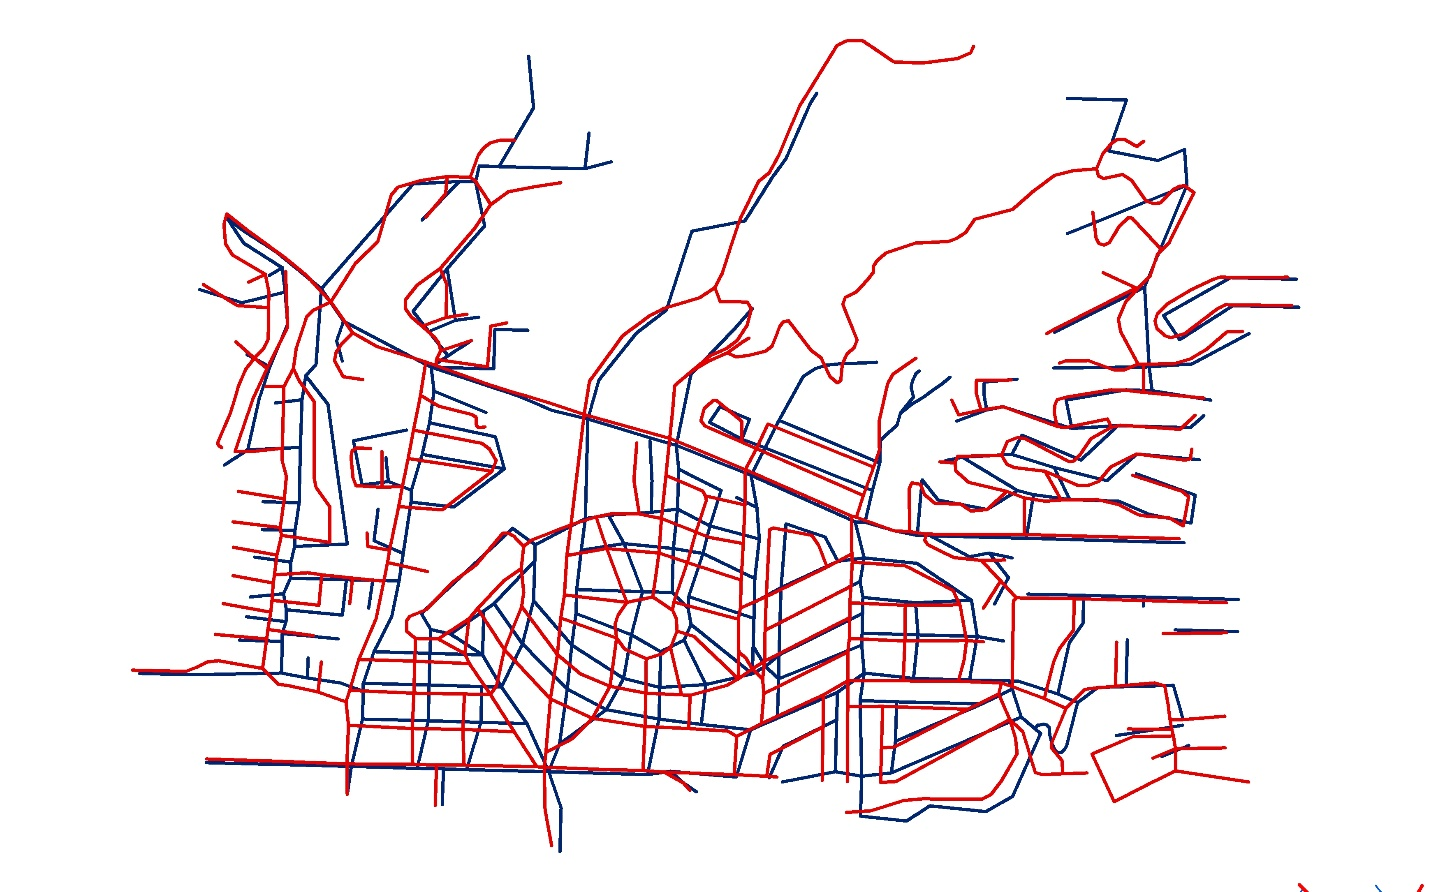
\includegraphics[scale=0.7]{memo_fig1.png}
\caption{Positional uncertainty: Street networks in Santa Barbara, CA from two different data sources}
\end{SCfigure}

\noindent \textbf{Precision} is another contributor to uncertainty. Modeling and methodologies used to collect data lead to this issue, for example, measuring temperature only three times per data to calculate the average temperature; using intervals such as population from 100 - 500 when recording the data. \textbf{Completeness}, \textbf{consistency} and \textbf{subjectivity} are all factors that causes low quality of spatial data. For most of the time, people tend to believe that the visualizations of GIS data are reliable, and interpret without thinking of the risk of uncertainty. Therefore, it is critical to represent existing uncertainties of spatial data in visuals. 

\section*{Strategies to Represent Uncertainty}
\noindent In general, methods to display uncertainty of spatial data are categorized as intrinsic and extrinsic mapping. As the name means, \textbf{extrinsic} strategy utilizes adjacent views or paired maps. The advantage of using paired map is preventing this extra dimension of information from cluttering with original views. This approach depends on the complexity of GIS dataset. When existing display includes more than four dimensions, an adjacent view or interactive graph will be a preferable choice. 

\begin{SCfigure}[][h]
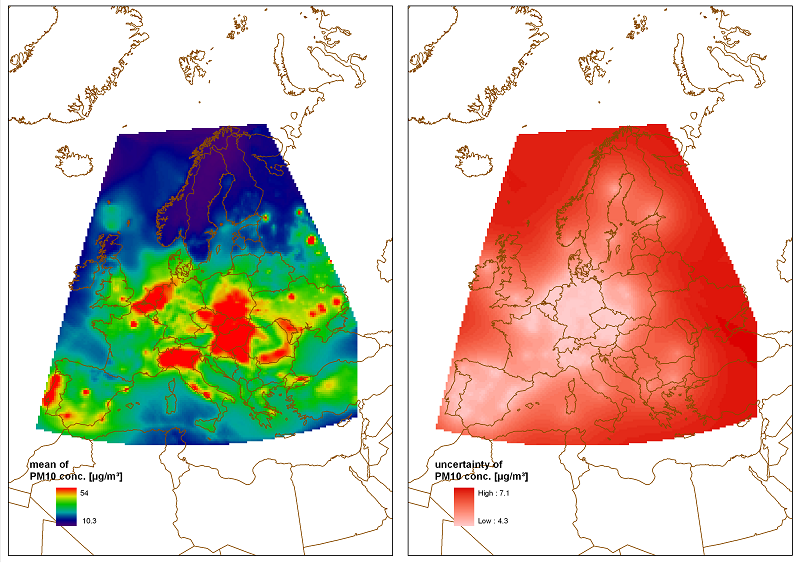
\includegraphics[scale=0.6]{memo_fig2.png}
\caption{A side-by-side map. Left one shows air pollution, the PM10 concentration in regions when another one showing related uncertainty. They are distinct by different color scale.}
\end{SCfigure}

\noindent Common \textbf{intrinsic} strategies to display levels of uncertainty is referring to the famous \textit{uncertainty visualization cube}, where each corner represents one way of distinction. They are distinctive color value (colors that fade out with higher levels of uncertainty), texture (coarser if uncertainty is high), location, transparency, and blurriness/fuzziness to represent data of regions with high or low uncertainty. These methods can be easily applied by adding layers of geom points or polygons on original graph.

\begin{figure}[h!]
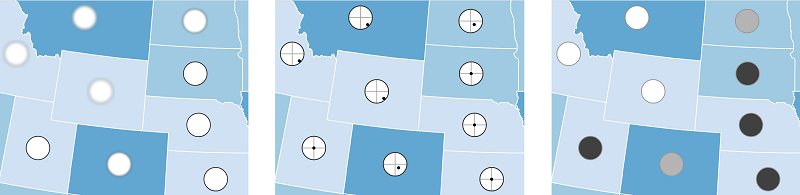
\includegraphics[scale=0.75]{memo_fig3.png}
\caption{left: fuzziness/blurriness. center: location. right: color value \\
These three visual variables have relatively high intuitive for representing levels of uncertainty}
\end{figure}

\noindent Extensive user study by MacEachren et al. about the intuitiveness of encoding for uncertainty visualization found most of these visual variables link to a visual metaphor that evokes the idea of uncertainty. Base on his research, fuzziness, location, and color value (as shown in the graph) have highest rank among all variables. Considering both readability and intuitiveness, the above lists of visual variables are best choice to encode the idea of uncertainty in spatial data. \\


\noindent However, It is a complex procedure to comprehensively create representation of uncertainty, due to heterogeneity in types of uncertainty: variation in the data, precision, completeness and so on. For now, the best way to represent such complexity is to converge ways of representation, for example, use levels of blurriness to represent completeness, and location to display variations. Drawback of this approach is also clear. Adding too many layers will reduce the readability, confusing users to intuitively understand degrees of uncertainty. 

\section*{Example of Visualizing Uncertainty }
\begin{figure}[h]
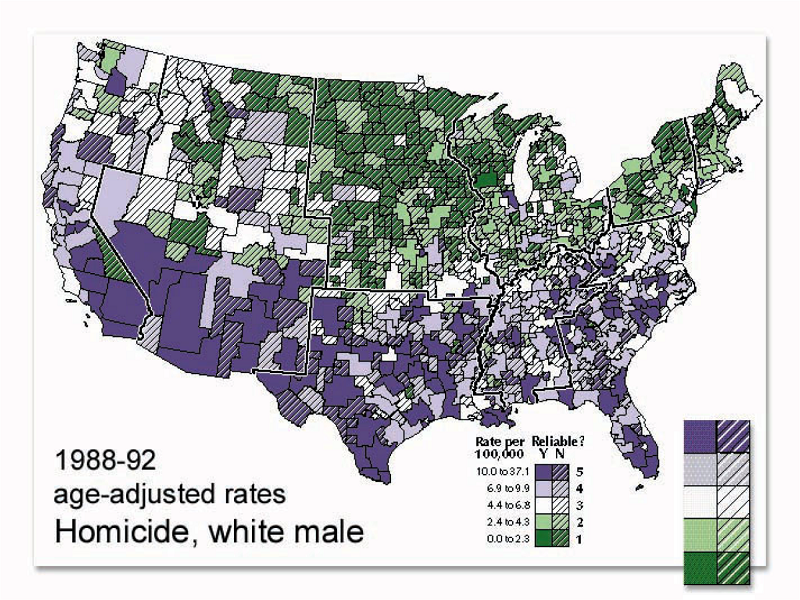
\includegraphics[scale=0.65]{memo_fig4.png}
\caption{This choropleth map shows homicide rates in US from 1988 to 1992. \\
Uncertainty values are marked by different texture.}
\end{figure}

\noindent Shadows on this map could only show logistic relationship (yes or no) in uncertainty values. Clearly, multiple types of uncertainty could be quantified in this case. Using blurriness or location could better display the 
variation among each group, accuracy and completeness of the dataset.

\section*{Works Cited}
\begin{enumerate}
\item Kinkeldey, C., \& Senaratne, H. (2018). Representing Uncertainty. The Geographic Information Science \& Technology Body of Knowledge (2nd Quarter 2018 Edition), John P. Wilson (ed.). \\
\item Li, L. (2017). Spatial data uncertainty. The Geographic Information Science \& Technology Body of Knowledge (4th Quarter 2017 Edition), John P. Wilson (ed).\\
\item Beard, M., Buttenfield, B., \& Clapham, S. (1991). NCGIA Research Initiative 7: Visualization of Spatial Data Quality, Scientific Report for the Specialists Meeting, NCGIA Technical Paper, 91-26, Santa Barbara, California. \\
\item Sanyal, J., S. Zhang, G. Bhattacharya, P. Amburn, \& Moorhead, R. (2009). A User Study to Compare Four Uncertainty Visualization Methods for 1D and 2D Datasets. IEEE Transactions on Visualization and Computer Graphics 15(6), 1209-1218. \\
\item MacEachren, A. M., Roth, R. E., O'Brien, J., Li, B., Swingley, D., \& Gahegan, M. (2012). Visual Semiotics \& Uncertainty Visualization: An Empirical Study, IEEE Transactions on Visualization and Computer Graphics, 18(12), 2496-2505.
\end{enumerate}



\section{Mapping Uncertainty}
\subsection*{Spatial Data Uncertainty}
Data uncertainty can be broadly divided into two categories, measurement error, and variation of data. When a map is created from GIS software, information loss is unavoidable. Measurement error directly lead to the difference between real geographic phenomenon and user's understanding. Therefore, informing viewer with accuracy and completeness of the spatial data that have been applied on visualization is important. Variation on event data is another cause of uncertainty. Mostly in research of environment and prediction, people tend to use mean value as representation of the event, for example, the mean daily temperature. It is obvious that temperature varies within the day, hence displaying uncertainty is a critical step to improve completeness of data communication. 

\subsection*{Strategies to Represent Uncertainty}
Whether adding uncertainty of data into the graph as additional information depends on kinds of the problem to solve. Generally, when working on model of prediction or using mean value as data point, visualizing uncertainty could generate new perspective and understanding. \\

In general, methods to display uncertainty are categorized as intrinsic and extrinsic mapping. Common intrinsic strategies to display levels of uncertainty is referring to the uncertainty visualization cube, where each corner represents one way of distinction. They are distinctive color value (fade out and fade in), texture (coarser or denser), transparency and fuzziness. These methods are not universally acceptable to all problems, in cases of more than two dimension of data, the addition layer that represents uncertainty might confuse viewer.  \\

In contrast, extrinsic strategy is the preferable choice for most of the cases. As the name means, extrinsic strategy utilizes adjacent views (paired maps) or small multiples which prevents extra dimension of data from cluttering with original views. This example of mean annual number of frost day around Spain. Righthand side displays mean values of frost and summer days, while righthand side are their corresponding uncertainty. In this case, uncertainty are range of the data. \\

\begin{figure}
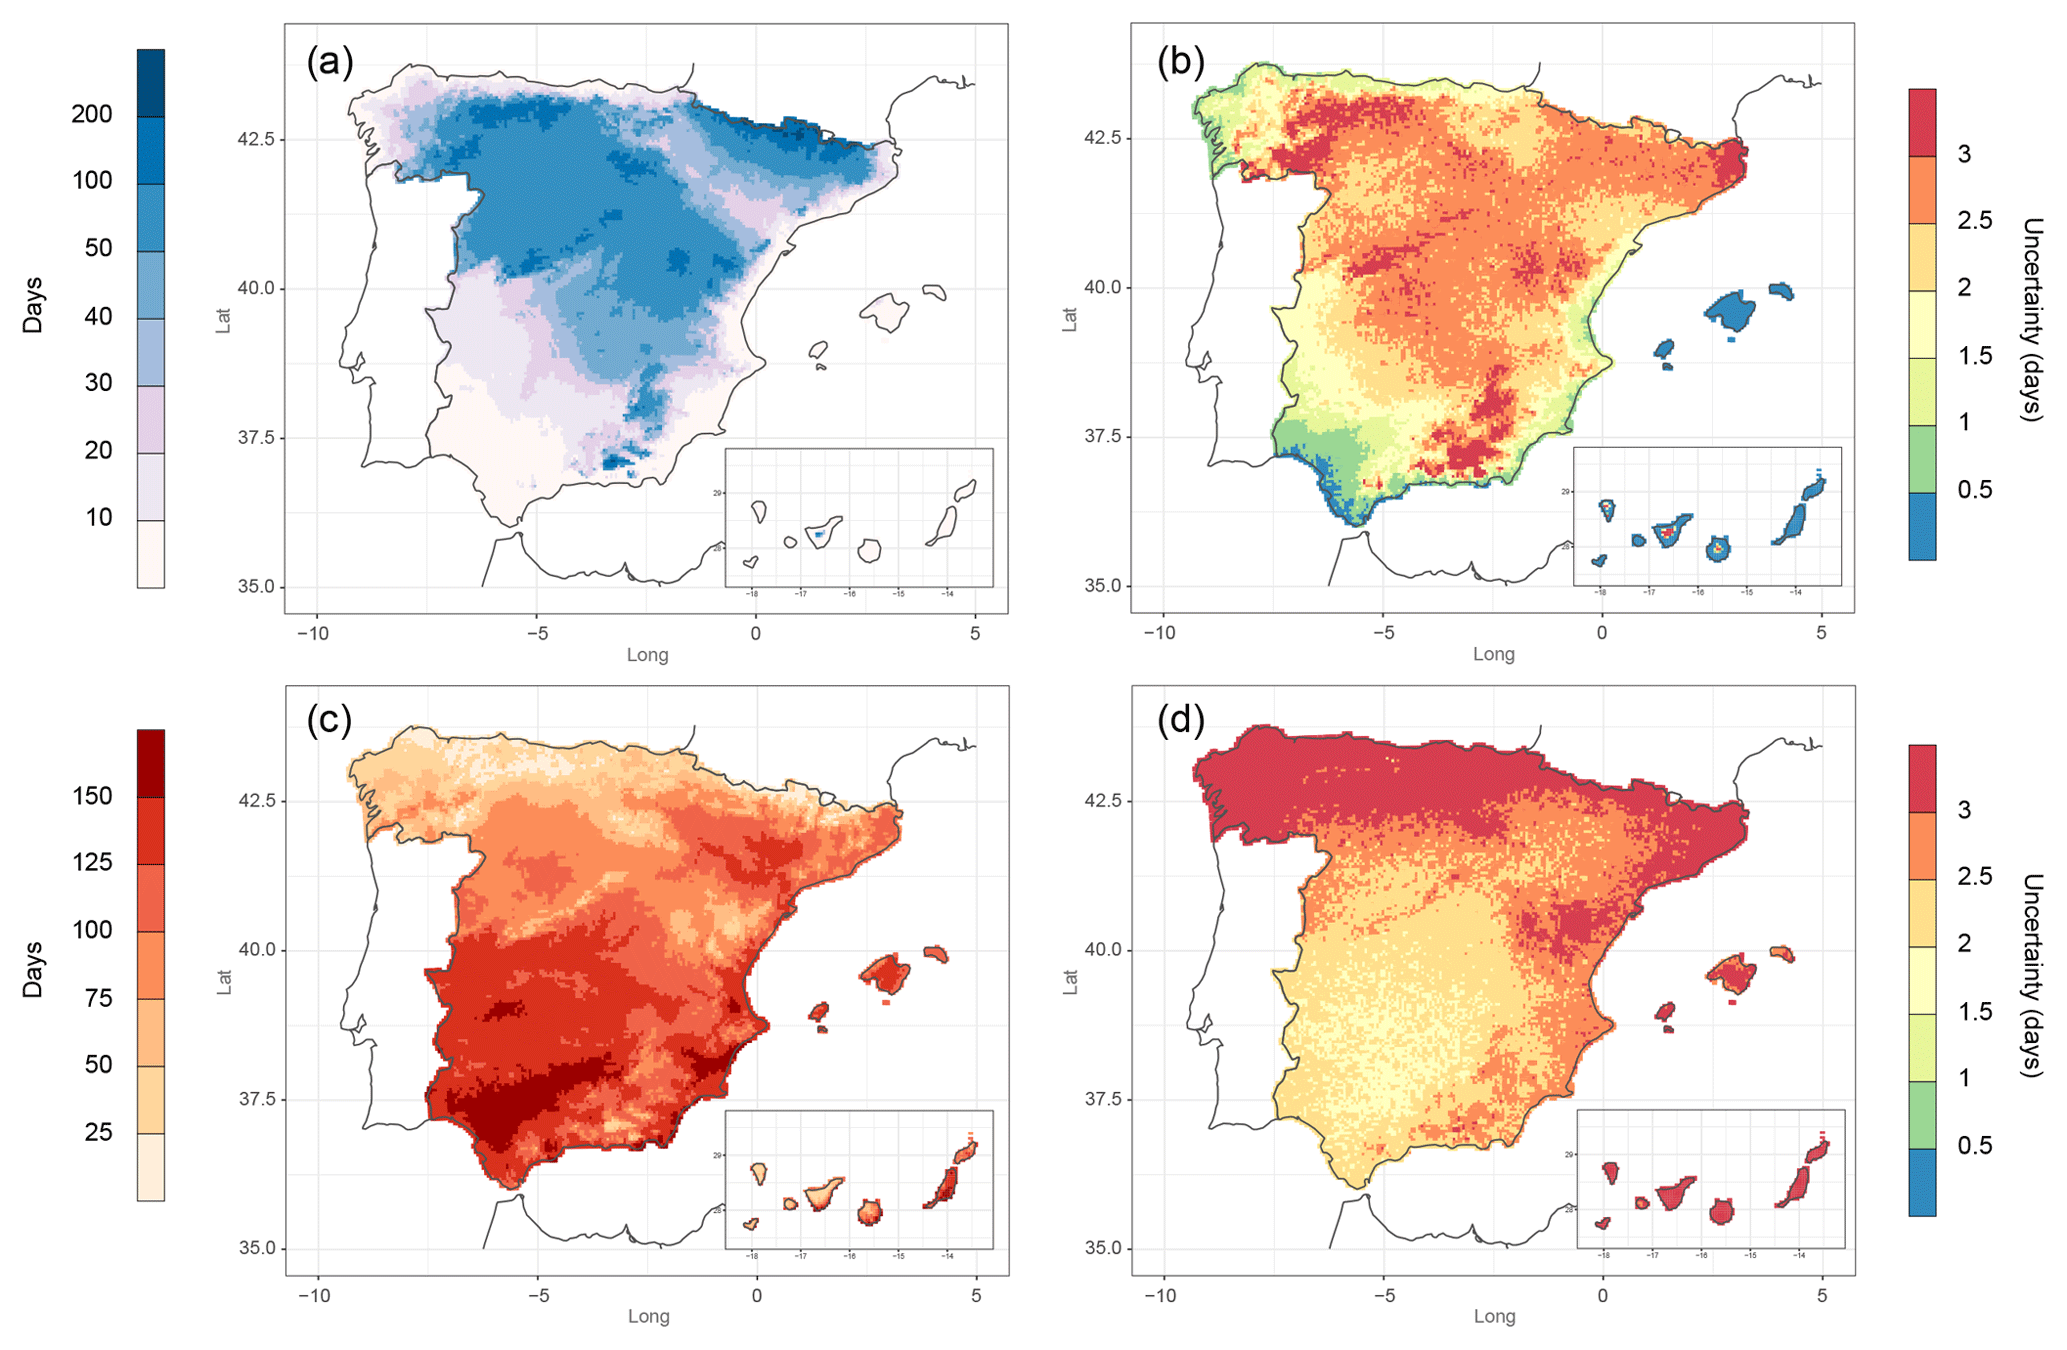
\includegraphics[width=6in]{uncertainty-2.png}
\caption{Uncertainty of Annual Frost and Summer Day}
\end{figure}






Using interactive system for large scale of map enables user to check the variation and bias for spacial data. This example of displaying prediction model of Above Ground Biomass (AGB) map takes into account error of random foresting model and the lidar model.

\begin{figure}
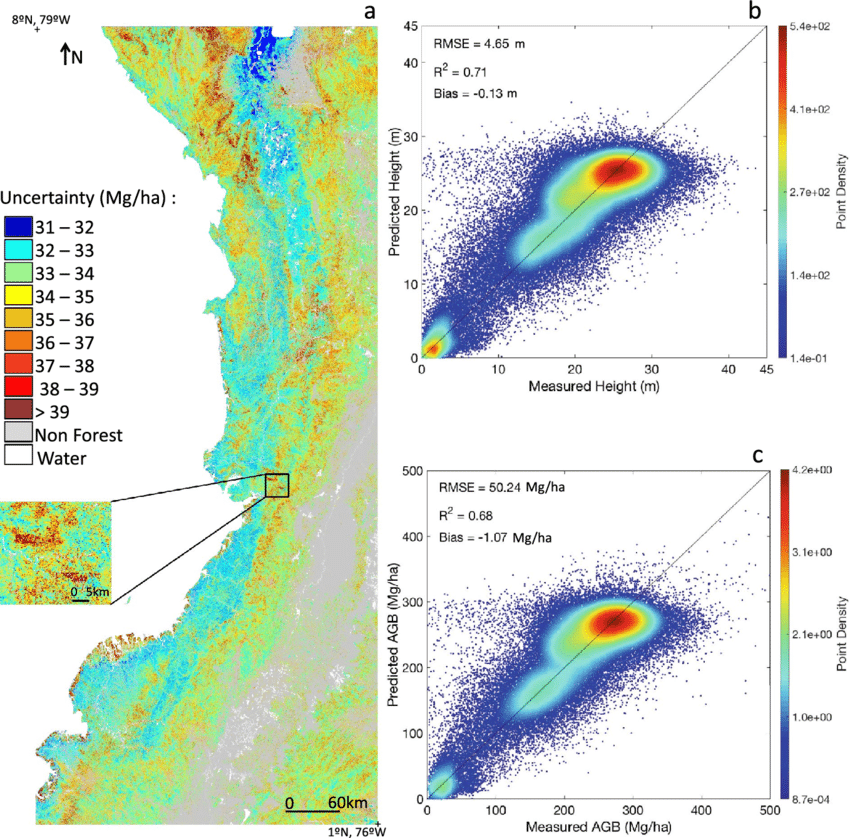
\includegraphics[width=6in]{uncertainty-1.png}
\caption{Uncertainty of AGB Map}
\centering
\end{figure}























\end{document}